\vspace{-0.1in}
\section{Network Designs for Disaggregation}
\label{sec:existing}
\vspace{-0.05in}
Our evaluation so far ignored the impact of queueing delay on end-to-end latency and hence application performance. We remedy the omission in this section.
The challenge is that queueing delay is a function of the overall network design, including: the traffic workload, network topology and routing, and the end-to-end transport protocol. Our evaluation focuses on existing proposals for transport protocols, with standard assumptions about the datacenter topology and routing (described below). However, the input traffic workload in \dis will be very different from that in a server-centric datacenter and, to our knowledge, no models exist that characterize traffic in a \dis. 

We thus start by devising a methodology that extends our experimental setup to generate an application-driven input traffic workload (\S\ref{ssec:ssmethod-traffic}), then describe how we use this traffic model to evaluate the impact of queueing delay (\S\ref{ssec:ssmethod}). Finally, we present our results on: (i) how existing transport designs perform under \dis traffic workloads (\S\ref{ssec:nlp}), and (ii) how existing transport designs impact end-to-end application performance (\S\ref{ssec:alp}). To our knowledge, our results represent the first evaluation of transport protocols for \dis. 

%
\eat{ 
SR:OSDI-CUT
\begin{figure*}
    \centering
    \subfigure[Total Traffic Volumes]{
        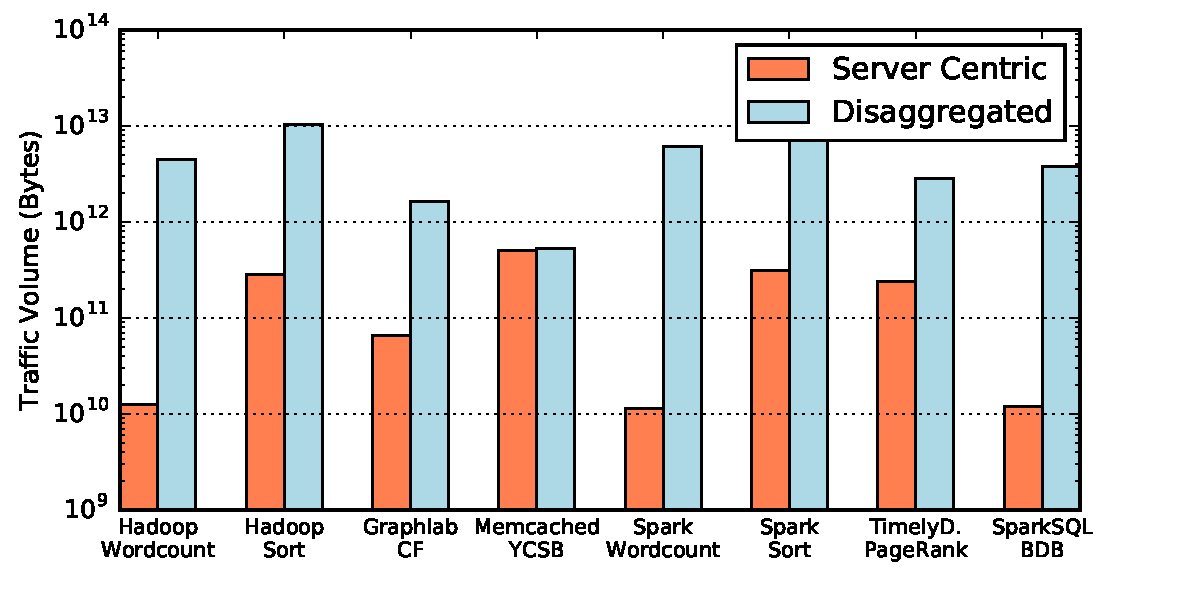
\includegraphics[width=0.95\columnwidth]{img/trafficVolume/trafficvolumes}
        \label{fig:trafvol:trafvols}
    }
    \subfigure[Temporal Traffic Volume Distribution]{
        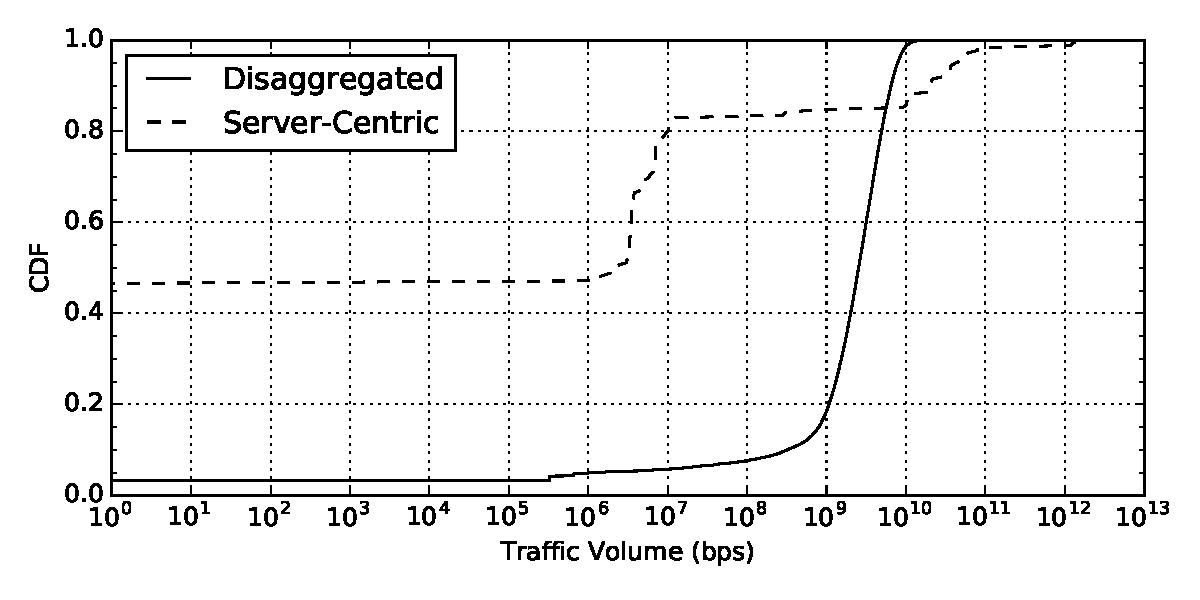
\includegraphics[width=0.95\columnwidth]{img/trafficVolume/temporalTraffic_cdf}
        \label{fig:trafvol:trafcdf}
    }
    \caption{\small{
    Figure~\ref{fig:trafvol:trafvols} compares traffic volumes between server centric and disaggregated datacenters. In almost all cases, the traffic volume increases by 1-2 orders of magnitude when moving from a server-centric to a disaggregated model; intuitively, CPU-memory and CPU-disk traffic that was previously contained within a server is now carried over the network. The obvious exception is memcached -- since most of the traffic in server-centric memcached corresponds to DRAM accesses, the traffic volume does not significantly increase.
    Figure~\ref{fig:trafvol:trafcdf} shows the distribution of traffic volumes for 100ms time intervals on the most highly loaded host while running the Spark Sort application. Note that for the disaggregated workload, the load over time is higher with disaggregation, but the tail load is lesser. Indeed, in the server centric workload, for almost half of the time intervals the link is quiescent.
    }}
    \label{fig:trafvol}
\end{figure*}
}
%
\vspace{-0.1in}
\subsection{Methodology: \dis Traffic Workloads}
\label{ssec:ssmethod-traffic}
\vspace{-0.05in}
Using our experimental setup from \S\ref{ssec:rmethod}, we collect a remote memory access trace from our instrumentation tool as described in \S\ref{ssec:rmethod}, a network access trace using {\tt tcpdump}~\cite{tcpdump}, and a disk access trace using the {\tt blktrace} utility.

We translate the accesses from the above traces to network flows 
in our simulated disaggregated cluster by splitting each node into one compute, one memory, and one disk blade and assigning memory blades to virtual nodes.

All memory and disk accesses captured above are associated with a specific address in the corresponding CPU's global virtual address space. We assume this address space is uniformly partitioned across all memory and disk blades reflecting our assumption of distributed data placement (\S\ref{ssec:system}).  

One subtlety remains. Consider the disk accesses at a server $A$ in the original cluster: one might view all these disk accesses as corresponding to a flow between the compute  and disk blades corresponding to $A$, but in reality $A$'s CPU may have issued some of these disk accesses in response to a request from a remote server $B$ (\eg, due to a shuffle request). 
In the disaggregated cluster, this access should be treated as a network flow between \emph{$B$}'s compute blade and $A$'s disk blade %SR:OSDI-CUT (i.e., the compute blade obtained by disaggregating server B and the disk blade that corresponds to disaggregating A).

To correctly attribute accesses to the CPU that originates the request, we match network and disk traces across the cluster -- e.g., matching the network traffic between $B$ and $A$ to the disk traffic at $A$ -- using a heuristic based on both the timestamps and volume of data transferred. 
If a locally captured memory or disk access request matches a local flow in our {\tt tcpdump} traces, then it is assumed to be part of a remote read and is attributed to the remote endpoint of the network flow.
Otherwise, the memory/disk access is assumed to have originated from the local CPU. 
%
\eat{
%SR: OSDI-CUT

Figure~\ref{fig:trafvol} plots a few characteristics of our resultant \dis traffic workload alongside that in the corresponding non-disaggregated architecture. As expected, disaggregation significantly changes the nature of the traffic workload, pointing to the importance of our characterization effort.
\pg{We omit Spark Streaming and HERD because Spark Streaming generates negligible remote memory traffic and HERD only works in single server mode in its current implementation.}
}

\vspace{-0.1in}
\subsection{Methodology: Queueing delay}
\label{ssec:ssmethod}
\vspace{-0.05in}
We evaluate the use of existing network designs for \dis in two steps.
First, we evaluate how existing network designs fare under \dis traffic workloads. 
For this, we consider a suite of state-of-the-art network designs and use simulation to evaluate their network-layer performance -- measured in terms of flow completion time (FCT) -- under the traffic workloads we generate as above.
We then return to actual execution of our applications (Table~\ref{tab:workloads}) and once again emulate disaggregation by injecting latencies for page misses. 
However, now we inject the flow completion times obtained from our best-performing network design (as opposed to the constant latencies from \S\ref{sec:requirements}). This last step effectively `closes the loop', allowing us to evaluate the impact of disaggregation on application-level performance for realistic network designs and conditions. 

\paragraphb{Simulation Setup}
For all the simulations in this section, we use the same setup as prior work on datacenter transport designs~\cite{pfabric, phost}. 
We simulate a %$144$-node (9 racks of 16 servers each) 
topology with 9 racks and a full bisection bandwidth Clos topology with $36$KB buffers per port; our two changes from prior work are to use $40$Gbps or $100$Gbps access links (as per ~\S\ref{sec:requirements}), and setting propagation and switching delays as discussed in \S\ref{ssec:rtt} (Table~\ref{tab:latency}).
%: 20 ns within a rack, 200ns for aggregation links, and a switching delay of 200ns per hop. 
We evaluate five protocols; in each case, we set protocol-specific parameters following the default settings but adapted to our bandwidth-delay product as recommended. Two protocols, TCP and DCTCP~\cite{dctcp}, see wide adoption today; the remaining three --- pFabric~\cite{pfabric}, pHost~\cite{phost}, and Fastpass~\cite{fastpass} --- are recent research proposals.

We evaluate both rack-scale and datacenter-scale traffic generation, where communicating nodes are constrained to be within a rack and unconstrained, respectively.

%
\begin{figure}[t]
  \centering
%    \subfigure[Datacenter-Scale Disaggregation]{
%      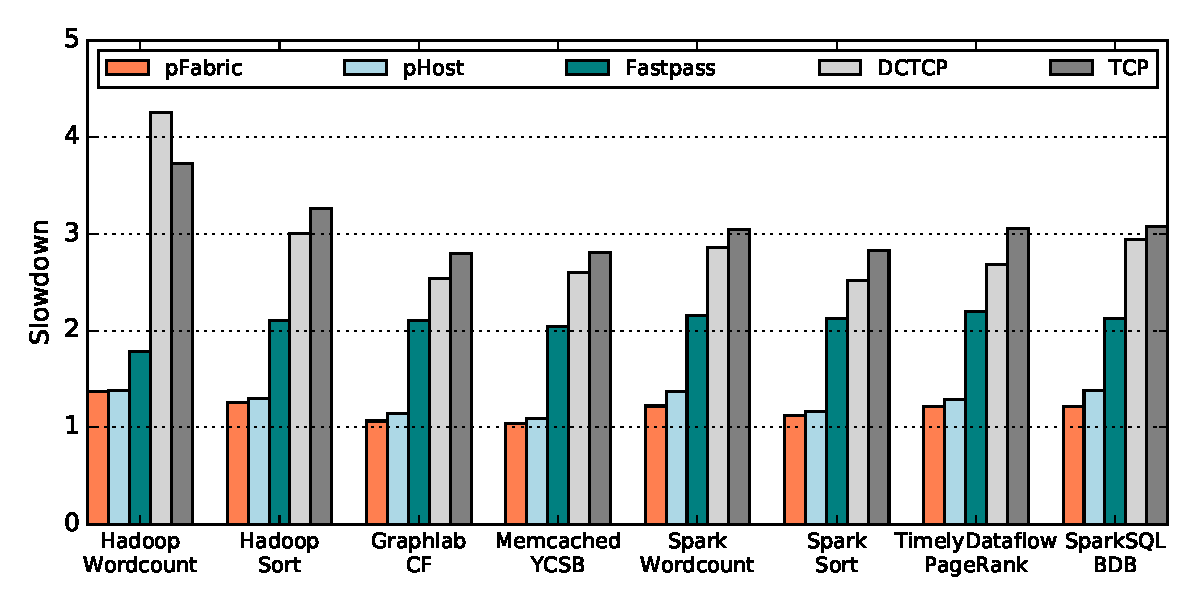
\includegraphics[width=\columnwidth]{img/slowdowns/100g/allFlows_dc-scale_slowdowns} 
%      \label{fig:phostp-dc}
%    }
%    \subfigure[Rack-Scale Disaggregation]{
      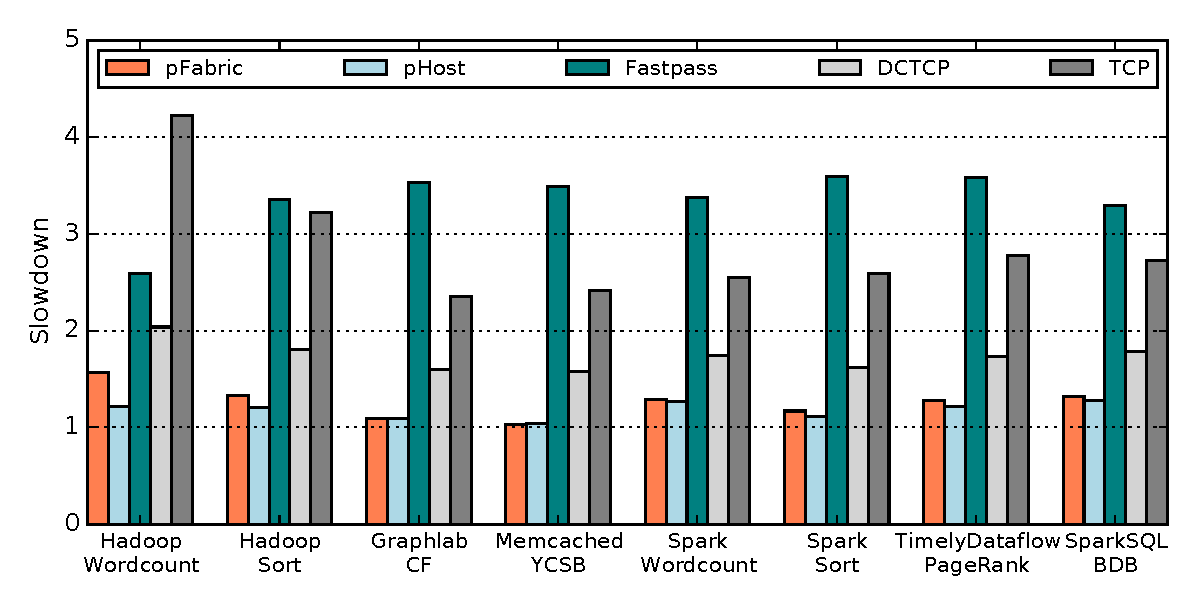
\includegraphics[width = 0.485\textwidth]{img/slowdowns/100g/allFlows_rack-scale_slowdowns} 
%      \label{fig:phostp-rs}
%    }
  \caption{\small{The performance of the five protocols for the case of $100$Gbps access link capacity. The results for $40$Gbps access links lead to similar conclusions. See \S\ref{ssec:nlp} for discussion on these results.}}
  \label{fig:phostp}
\end{figure}
%
\vspace{-0.1in}
\subsection{Network-level performance}
\label{ssec:nlp}
\vspace{-0.05in}
We evaluate the performance of our candidate transport protocols in terms of their  mean slowdown~\cite{pfabric}, which is computed as follows. The slowdown for a flow is computed by dividing the flow completion time achieved in simulation by the time that the flow would take to complete if it were alone in the network. The mean slowdown is then computed by averaging the slowdown over all flows.
Figure~\ref{fig:phostp} plots the mean slowdown for our five candidate protocols, using $100$Gbps links (all other parameters are as in \S\ref{ssec:ssmethod}). 

\paragraphb{Results} 
We make the following observations. 
First, while the relative ordering in mean slowdown for the different protocols is consistent with prior results~\cite{phost}, their \emph{absolute} values are higher than reported 
in their original papers; e.g. pFabric and pHost both report close-to-optimal slowdowns with values close to 1.0~\cite{phost,pfabric}. 
%And this is true even though the average network utilization in our \dis workload is in fact substantially lower than the utilization levels used in the simulation studies of ~\cite{pfabric, phost}. 
On closer examination, we found that the higher slowdowns with disaggregation are a consequence of the differences in our traffic workloads (both earlier studies used heavy-tailed traffic workloads based on measurement 
studies from existing datacenters). In our \dis workload, reflecting the 
application-driven nature of our workload, we observe many flow arrivals that 
appear very close in time (only observable on sub-10s of microsecond timescales), leading to high slowdowns for these flows. This effect is strongest in the case of the wordcount application which is why it suffers the highest slowdowns. 
We observed similar results in our simulation of rack-scale disaggregation (graph omitted).

\eat{
%SR: OSDI-CUT

Second, we note that while pFabric and pHost perform comparably, Fastpass fares worse; this is consistent with the findings reported in~\cite{phost}.

Finally, we repeat the above simulations but this time simulate rack-scale 
disaggregation; \ie, a CPU blade's associated memory and disk blades are selected from 
its own rack. The results are shown in Figure~\ref{fig:phostp}. We see that, with the exception of Fastpass, rack-scale disaggregation does not significantly alter the slowdown values. (Fastpass fares worse with rack-scale disaggregation because the centralized scheduler is not rack-local and hence the cost of contacting the scheduler is relatively greater.)
However, one should not conclude from this that rack-scale containment is not useful because our slowdown metric masks differences in the \emph{absolute} FCT values. Instead, slowdown is useful primarily to compare across different transport protocol designs. The impact of these absolute FCT values is captured in our next experiments.
}

\vspace{-0.1in}
\subsection{Application-level performance}
\label{ssec:alp}
\vspace{-0.05in}
We now use the FCTs obtained from the above simulations as the memory access times in our emulation methodology from \S\ref{sec:requirements}. We use the FCTs from pFabric as it achieves the best slowdowns over a range of test scenarios. 

We measure the degradation in application performance that results from injecting remote memory access times drawn from the FCTs that pFabric achieves with 40Gbps links and with 100Gbps links, in each case considering both datacenter-wide and rack-scale disaggregation. As in \S\ref{sec:requirements}, we measure performance degradation compared to the baseline of performance without disaggregation (i.e., injecting zero latency). 

In all cases, we find that the inclusion of queueing delay \emph{does} have a non-trivial impact on performance degradation -- typically increasing the performance degradation relative to the case of zero-queueing delay by between 2-3x. 
Figure~\ref{fig:appfabric100} plots the performance degradation for 100Gbps links: we see that degradation ranges between 1-8.5\% on average with datacenter scale disaggregation, and containment to a rack lowers the degradation to between 0.4-3.5\% on average. In topologies with 40Gbps links, we find a median performance degradation of 17\% with datacenter-scale disaggregation (figure not shown). 
This leads us to conclude that 100Gbps links are both required and sufficient to contain the performance impact of queueing delay.

%
\begin{figure}
  \centering
    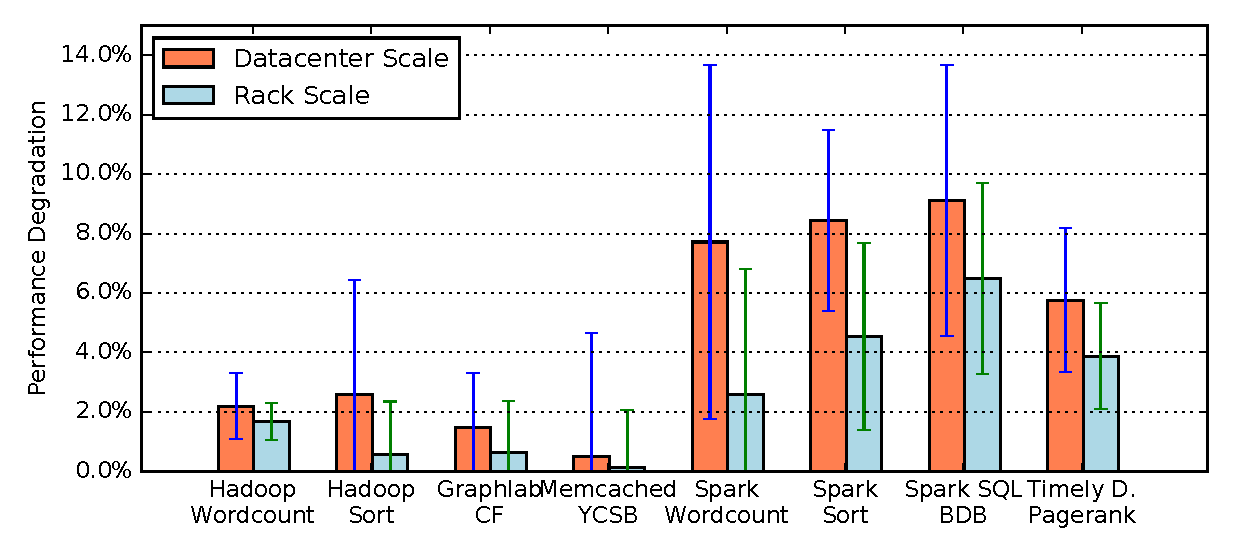
\includegraphics[width = \columnwidth]{img/slowdown.eps} 
  \caption{\small{Application layer slowdown for each of the four applications at rack-scale and datacenter scale after injecting pFabric's FCT with 100Gbps link. }}
  \label{fig:appfabric100}
\end{figure}
%

\vspace{-0.1in}
\subsection{Low latency remote memory}
\vspace{-0.05in}
\rc{
As we have established in the previously section, a DDC requires 100Gbps bandwidth and 3-5us end-to-end latency. 
Current datacenter network usually has 20us network latency, and by our analysis, 5-7us of end-to-end latency is within reach. 
If we enable RDMA inside the datacenter, which takes aways the overhead at OS layer, we can get latency as low as 3-5us. 
We validate this by building a kernel space RDMA block device driver, and use this block device driver as the swap device.
With the RDMA block device driver, the local machine can swap to remote memory instead of swapping to disk.

We implement the block device driver on a machine with Mellanox  4xFDR Infiniband card.
To maintain high throughput, we first use a batch implementation that batches block requests and sends all of them together to the RDMA NIC.
The driver waits for all the request to come back and notify the upper layer.
We test the block device throughput using \textit{dd} with direct IO, and measure the request latency by instrumenting the driver code.
The block device throughput is only 0.8GB/s and the latency is around 4-16us.
We observed that many block requests are actually contiguous in address, so we merge these request in to one large request. 
With request merging, the throughput becomes 2.6GB/s, which is ~3x better than the batch version. 
The performance of the block device driver can be further improved by issuing RDMA requests asynchronously.
We create a data structure to keep track of all the out going requests and notify the upper layer immediately for each completed request.
This improves the throughput to 3.3GB/s which is as high as a local RamFS, and reduces the request latency to 3-4us (Table \ref{tab:rdma_latency}).

\begin{table}[t]
    \centering
    \small
    \begin{tabular}{ccccc}
    \textbf{Min}	& \textbf{Avg}	& \textbf{Median} & \textbf{99.5 Pcntl}	& \textbf{Max}\\
    \hline
    3394 &	3492&	3438&	4549&	12254\\\hline
    \end{tabular}
    \caption{RDMA block device request latency(ns)}
    \label{tab:rdma_latency}
\end{table}

In current non-NUMA architecture, Linux Kernel only launches one \textit{kswapd} to swap out least recently used pages. 
This could be a bottleneck for apps that heavily use remote memory.
We enable the NUMA\_EMU feature in Linux kernel, which partitions the memory into several regions, and each memory region gets its own \textit{kswapd}. 
This improves the throughput of swapping out memory pages.


The RDMA block device driver provides us a simple and efficient way utilize remote memory. 
We setup the block device as swap space and run the \rc{5} applications evaluated in \S \ref{sec:requirements} with lower latency requirements.
\rc{waiting for joao's results}

}
\rc{
\paragraphb{Measuring swap latency}
We measured the software overhead of swapping on a commodity desktop running
Linux 3.13.0. In order to do so, we needed to collect two data points with
minimal modifications to the codebase --- the overall time spent in the page
fault handler on a swap and the time spent actually accessing disk. Although
convenient measurement tools such as \texttt{ftrace} exist, they introduced
unacceptable overhead for our purposes. We also could not arbitrarily introduce
\texttt{printk} calls within the areas we were measuring, since \texttt{printk}
introduces a noticable overhead when measuring on the order of microseconds. In
order to perform the measurement, we took advantage of the fact that the
\texttt{handle\_mm\_fault} function called by the page fault handler (and which
eventually handles swaps) never utilizes the upper 16 bits of its 32 bit return
value, as evidenced by the \texttt{VM\_FAULT\_*} macros in the \texttt{mm.h}
header.

Thus, we wrap both the body of the \texttt{\_\_do\_page\_fault} function and the
call to the \texttt{swapin\_readahead} function (which performs a swap from
disk) in ktime\_get calls.  We then pack the result of the measurement for the
swapin\_readahead function into the upper 16-bits of its caller,
\texttt{do\_swap\_page}, which propagates the value up to
\texttt{\_\_do\_page\_fault}. Once we have completed measuring the body of
\texttt{\_\_do\_page\_fault}, we print both the latency of the whole
\texttt{\_\_do\_page\_fault} routine, as well as the time spent in
\texttt{swapin\_readahead}. We subtract these and average to find that the
software overhead of page fault handler is around 20.5 microseconds. This
number is a lower-bound on the software overhead of the handler, because we
assume that all of swapin\_readahead is a ``disk access''. This is due to the fact
that we cannot neatly instrument inside swapin\_readahead in the same manner
since it returns a pointer.

Overall, our measurement code introduces a very small number of bitwise
operations (ANDs, ORs, shifts), one integer subtraction, and four calls to
\texttt{ktime\_get} into the handler, which together have a negligible impact on
measurements.
}